\documentclass[a4paper]{article}
\usepackage[margin=1in]{geometry}
\usepackage[T1]{fontenc}
\usepackage[utf8]{inputenc}
\usepackage[hidelinks]{hyperref}
\usepackage{amsmath, amssymb, amsthm}
\usepackage{graphicx}
\usepackage{listings}
\usepackage{xcolor}
\usepackage{booktabs}
\usepackage{caption}

% Configuration pour les listings de code
\definecolor{codebg}{RGB}{245,245,245}
\lstset{
    backgroundcolor=\color{codebg},
    basicstyle=\ttfamily\small,
    frame=single,
    breaklines=true,
    columns=fullflexible,
    keywordstyle=\color{blue},
    commentstyle=\color{gray},
    stringstyle=\color{orange},
    showstringspaces=false
}

%----- TITLE PAGE INFO -----%
\title{\Huge \textbf{Spanning Tree Protocol (STP) Workbook}\\
       \Large Fundamentals, Variants, Tuning, and Practical Labs}
\author{\Large Written for Networking Students and Professionals}
\date{\today}

\begin{document}

%----- MODERN TITLE PAGE -----%
\begin{titlepage}

    \centering
    \vspace*{4cm}
    {\Huge \textbf{EtherChannel}\par}
    \vspace{0.8cm}
    {\Large A Hands-On Guide to PAgP, LACP, and Static Aggregation\par}
    \vspace{0.3cm}
    \rule{0.9\textwidth}{1pt}
    
    \vspace{0.6cm}
    {\large \textbf{Mehdi JAFARI ZADEH}}\par
    \vspace{0.3cm}
	\centering
	\vspace*{4cm}

	\vfill
	\textbf{Date:} \today
	\vspace{2cm}
\end{titlepage}

\tableofcontents
\newpage
\section{Introduction to EtherChannel}
In modern networking, \textbf{bandwidth, redundancy, and efficient link utilization} are critical components for maintaining high-performance and resilient network infrastructures. \textbf{EtherChannel} is a link aggregation technology that enables multiple physical Ethernet links to be combined into a single logical connection, increasing throughput and providing fault tolerance.

\subsection{What is EtherChannel?}
EtherChannel is a \textbf{Cisco-proprietary technology} that allows multiple physical Ethernet interfaces to be bundled together to function as a \textbf{single logical interface}. This aggregation increases bandwidth between switches, routers, and servers while also \textbf{enhancing redundancy and load balancing}. In the event of a single link failure, traffic is automatically redistributed across the remaining links without disrupting network communication.

\subsection{Key Benefits of EtherChannel}
\begin{enumerate}
    \item \textbf{Increased Bandwidth:} By combining multiple physical links, EtherChannel effectively multiplies available bandwidth.
    \item \textbf{Redundancy \& High Availability:} If one link in the bundle fails, traffic seamlessly continues over the remaining active links.
    \item \textbf{Load Balancing:} Traffic is distributed across all links in the EtherChannel, optimizing performance.
    \item \textbf{Reduced CPU Overhead:} Since EtherChannel is seen as a \textbf{single logical interface}, the switch CPU does not need to process multiple STP calculations.
    \item \textbf{Faster Convergence:} Unlike Spanning Tree Protocol (STP), which may take time to transition ports after a failure, EtherChannel \textbf{keeps the logical interface up} even when individual links fail.
\end{enumerate}

\subsection{EtherChannel Protocols}
EtherChannel can be established using different negotiation protocols:
\begin{itemize}
    \item \textbf{Port Aggregation Protocol (PAgP):} A Cisco-proprietary protocol that dynamically negotiates EtherChannel formation.
    \item \textbf{Link Aggregation Control Protocol (LACP):} An industry-standard (IEEE 802.3ad) alternative to PAgP that allows multi-vendor compatibility.
    \item \textbf{Static Mode (On Mode):} EtherChannel can be manually configured without negotiation, but this can lead to issues if not configured correctly on both sides.
\end{itemize}

\subsection{EtherChannel in Network Design}
EtherChannel is widely used in network infrastructures, including:
\begin{itemize}
    \item \textbf{Switch-to-Switch connections} to improve backbone connectivity.
    \item \textbf{Switch-to-Router connections} for faster inter-VLAN routing.
    \item \textbf{Server Redundancy \& Load Balancing} in data centers.
\end{itemize}

By implementing EtherChannel, network administrators can \textbf{optimize link usage, prevent bottlenecks, and improve overall network reliability}.

\newpage
\textbf{Etherchannel topology:}
\vspace{4cm}
\begin{figure}[h]
	\centering
	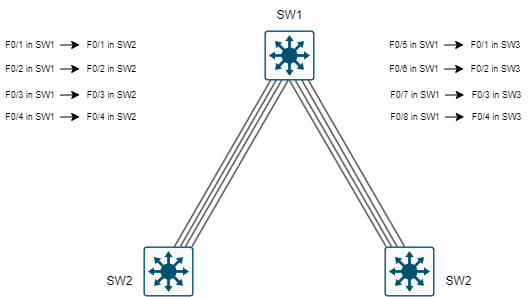
\includegraphics[width=0.9\textwidth]{img/Aggrigation-manual-01.png}
	\caption{\textit{}}
\end{figure}
\newpage
\section{EtherChannel Protocols}
\subsection{Configuring PAgP-based EtherChannel}
\begin{enumerate}
    \item Configure an \textbf{EtherChannel using PAgP} between SW1 and SW2 using interfaces F0/1 - F0/4.
    \item Verify the EtherChannel status using \texttt{show etherchannel summary} and interpret the output.
    \item What happens if one of the links in the EtherChannel fails? Test and analyze.
\end{enumerate}

\subsection{Exercise 2.2: Configuring LACP-based EtherChannel}
\begin{enumerate}
    \item Configure an \textbf{EtherChannel using LACP} between SW1 and SW3 using interfaces F0/5 - F0/8.
    \item Change the configuration to use \textbf{LACP Active mode} and check if the channel is formed.
    \item What is the difference between \textbf{LACP Active} and \textbf{LACP Passive}?
\end{enumerate}

\subsection{Exercise 2.3: Configuring Static Mode EtherChannel}
\begin{enumerate}
    \item Configure an \textbf{EtherChannel in Static Mode (On Mode)} between SW2 and SW3.
    \item What is the primary risk of using Static Mode instead of PAgP or LACP?
    \item Verify the configuration and discuss any errors you encounter.
\end{enumerate}

\subsection{Exercise 2.4: Comparing PAgP, LACP, and Static Mode}
\begin{enumerate}
    \item Create a comparison table highlighting the \textbf{differences between PAgP, LACP, and Static Mode}.
    
    \begin{tabular}{|l|l|l|l|}
        \hline
        Feature & PAgP & LACP & Static Mode \\
        \hline
        Protocol Type & Cisco proprietary & IEEE 802.3ad & None \\
        Negotiation & Active/Desirable & Active/Passive & Disabled \\
        Error Detection & Yes & Yes & No \\
        \hline
    \end{tabular}
    
    \item Based on the network topology, which EtherChannel mode would you recommend for maximum reliability?
\end{enumerate}

\section{Configuring EtherChannel}
\subsection{Exercise 3.1: Full EtherChannel Configuration}
\begin{enumerate}
    \item Configure \textbf{EtherChannel using LACP on SW1 \& SW2} (Interfaces F0/1 - F0/4).
    \item Configure \textbf{EtherChannel using PAgP on SW1 \& SW3} (Interfaces F0/5 - F0/8).
    \item Verify that all EtherChannels are up using \texttt{show etherchannel summary}.
    \item What does the status flag "SU" indicate in the \texttt{show etherchannel summary} output?
\end{enumerate}

\section{Load Balancing in EtherChannel}
\subsection{Exercise 4.1: EtherChannel Load Balancing Methods}
\begin{enumerate}
    \item Configure SW1 to use \textbf{Layer 2 Load Balancing} for EtherChannel.
    \item Change the configuration to \textbf{Layer 3 Load Balancing} and test using pings.
    \item Use \texttt{show etherchannel load-balance} to verify load balancing mode.
    \item Which load balancing method is best for environments with \textbf{heavy Layer 3 traffic}?
\end{enumerate}

\section{EtherChannel and VLANs}
\subsection{Exercise 5.1: Configuring VLANs with EtherChannel}
\begin{enumerate}
    \item Configure \textbf{VLAN 10 and VLAN 20} on SW1, SW2, and SW3.
    \item Assign VLAN 10 to \textbf{EtherChannel between SW1 and SW2}.
    \item Assign VLAN 20 to \textbf{EtherChannel between SW1 and SW3}.
    \item Verify VLAN configuration with \texttt{show vlan brief}.
\end{enumerate}

\subsection{Exercise 5.2: EtherChannel with Trunking}
\begin{enumerate}
    \item Configure the EtherChannel between SW1 and SW2 as a \textbf{trunk port}.
    \item Allow \textbf{only VLANs 10 and 20} on the trunk.
    \item Verify trunking using \texttt{show interfaces trunk}.
\end{enumerate}

\subsection{Exercise 5.3: VLAN Load Distribution}
\begin{enumerate}
    \item Configure VLAN load balancing on EtherChannel using \textbf{MAC address-based hashing}.
    \item Change the hashing method to \textbf{IP-based} and test using pings from multiple VLANs.
\end{enumerate}

\subsection{Exercise 5.4: Troubleshooting VLAN and EtherChannel Issues}
\begin{enumerate}
    \item Intentionally misconfigure VLANs in EtherChannel and analyze error messages.
    \item Use \texttt{show spanning-tree} to check if there are blocked ports.
    \item What happens if VLANs are not allowed on both EtherChannel sides?
\end{enumerate}

\section{Advanced EtherChannel Troubleshooting}
\subsection{Exercise 6.1: Identifying Common Problems}
\begin{enumerate}
    \item Configure EtherChannel with \textbf{one mismatched mode} (PAgP on one switch and LACP on the other).
    \item Analyze the \textbf{error messages} and explain why EtherChannel fails.
    \item How does EtherChannel react when one switch is powered off?
\end{enumerate}

\subsection{Exercise 6.2: Using Show Commands}
\begin{enumerate}
    \item Use \texttt{show etherchannel summary} and analyze the output.
    \item Use \texttt{show spanning-tree} to verify how STP interacts with EtherChannel.
    \item Use \texttt{debug etherchannel} to track EtherChannel negotiation.
\end{enumerate}

\subsection{Exercise 6.3: Best Practices in Troubleshooting}
\begin{enumerate}
    \item What are the three most common reasons for EtherChannel failure?
    \item How can \textbf{Port Speed/Duplex mismatches} affect EtherChannel?
    \item What steps should you take if an EtherChannel is \textbf{partially up}?
\end{enumerate}

\subsection{Exercise 6.4: Real-World Case Study}
\begin{enumerate}
    \item Read the following network issue scenario and propose a solution:
    \begin{itemize}
        \item "EtherChannel between SW1 and SW2 goes down when adding a new link. Removing the link restores the channel."
        \item What is the most likely cause?
        \item How can you prevent this from happening?
    \end{itemize}
\end{enumerate}

\section{EtherChannel in Data Center Networks}
\subsection{Exercise 7.1: MLAG vs. vPC}
\begin{enumerate}
    \item Research \textbf{Multi-Chassis Link Aggregation (MLAG) and vPC}.
    \item Compare them with traditional EtherChannel.
    \item Which method would be best for \textbf{redundancy in a data center}?
\end{enumerate}

\subsection{Exercise 7.2: Configuring vPC on Cisco Nexus}
\begin{enumerate}
    \item List the \textbf{steps to configure vPC} on Cisco Nexus devices.
    \item How does vPC differ from standard EtherChannel?
\end{enumerate}

\subsection{Exercise 7.3: Troubleshooting vPC}
\begin{enumerate}
    \item What is a \textbf{vPC orphan port}?
    \item How can a \textbf{vPC peer-link failure} impact a data center network?
    \item Provide solutions to avoid \textbf{vPC-related outages}.
\end{enumerate}

\section{Best Practices and Security Considerations}
\subsection{Exercise 8.1: EtherChannel Best Practices}
\begin{enumerate}
    \item List five best practices for deploying EtherChannel in a production network.
    \item What are the risks of \textbf{misconfigured EtherChannel}?
\end{enumerate}

\subsection{Exercise 8.2: Security Risks}
\begin{enumerate}
    \item How can EtherChannel be exploited in a \textbf{MAC spoofing attack}?
    \item What security measures can prevent \textbf{EtherChannel-based attacks}?
\end{enumerate}

\subsection{Exercise 8.3: Securing EtherChannel Configurations}
\begin{enumerate}
    \item Configure \textbf{BPDU Guard} and \textbf{Root Guard} on EtherChannel links.
    \item Why is \textbf{STP Loop Protection} important in an EtherChannel environment?
\end{enumerate}

\subsection{Exercise 8.4: Future Trends}
\begin{enumerate}
    \item Research new advancements in \textbf{Link Aggregation technologies}.
    \item How do \textbf{SDN and automation} impact EtherChannel deployment?
\end{enumerate}

\section{Final Exam: EtherChannel Deployment Challenge}
\begin{enumerate}
    \item Given a new topology, configure EtherChannel using the \textbf{best protocol} for redundancy.
    \item Implement \textbf{VLAN trunking and load balancing}.
    \item Troubleshoot an \textbf{EtherChannel failure scenario} and document the fix.
\end{enumerate}
\end{document}
